\begin{figure}[h]
\textbf{Tema d'Esame di Gennaio 2018}\\ \\
Una massa $M = 100 g$ viene lanciata con un sistema come quello in figura. Se la costante elastica della molla è $k = 500 N/m$, quale deve
essere la sua compressione perché la massa $M$ raggiunga un’altezza massima
$h = 2.00 m$ da terra. Il tratto inclinato forma un angolo $\theta$ = 20.0$^{\circ}$ con il terreno, è lungo $L = 50.0 cm$ e ha un coefficiente di attrito $f = 0.10$
\\
	\begin{center}
		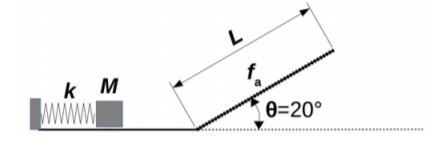
\includegraphics[scale=0.8]{ES2/GEN022018.jpg}
	\end{center}
	\noindent\fbox{
            \parbox{\textwidth}{
                \null\hfill \textbf{Soluzione:} $ \Delta x=0.09m $\\
                \textbf{Procedimento: } \\
				Trasformare le unità di misura:\\
				$ m= 100g=0.1kg$\\
                $\Delta s= 50cm =0.5m$\\ \\  
                Impostando il seguente sistema, considerando come punto A la molla ed il punto B al punto di masssima altezza (in cui si ferma).\\
				$U_{El,A} - L_a = U_B$ \\
				$\frac{1}{2}\cdot k \cdot \Delta x^2 - \mu_d \cdot m \cdot g \cdot cos(\alpha) \cdot \Delta s = m \cdot g \cdot h$\\
				$250N/m \cdot \Delta x^2= 0.046J + 1.962J \qquad \Delta x=\sqrt{\frac{2.008J}{250N/m}}=\sqrt{0.008m^2}=0.09m$\\ \\ 

                \textbf{Nota:} Questo esercizio in questo appello aveva dei dati sbagliati, pertanto una soluzione di questo genere sarebbe stata considerata valida nonostante non risolva il problema (si trasformava in un moto proiettile)
            }
        } 
\end{figure}